%!TEX root = ../sig-alternate.tex
\section{Data Collection, Cleansing and Insights}
\label{sec:dataset}

Our data set consists of data collected from Twitter between September 2009 and April 2015. It consist of 240 petitions that were part of climate change or animal welfare public campaigns spanning over 1300 tweets.

\textbf{Campaigns dataset and petition tweets:}
% * Environmental campaigns on Twitter and their collection by means of power users and crowdsourcing.
In order to analyze petitions role in the frame of climate change and animal welfare campaigns we have obtained an annotated corpus of such hashtags.
The corpus consists of 118 public campaigns with over 4M unique tweets (not including retweets) that spans over Feb 2009 - April 2015. Moreover, all the campaign hashtags are labeled by (a) high-level goal (awareness or mobilization) and (b) user engagement patter over time (one-day campaigns, ever-growing, annual, inactive etc)\footnote{One-day campaigns have the most user activity fallen into the start/first mention of the hashtag. Ever-growing campaigns have constantly growing number of users posting with the hashtag. Annual campaigns are mentioned annually, e.g., yearly, monthly. Inactive campaigns have very low user engagement overall.}.
Those are the main categories that will be used further in the analysis of petition positioning across various types of campaigns.

% * Elimination of duplicates and merge unobvious duplicates
Having the collection of environmental campaign tweets, we have identified all tweets with a mention of the ``petition''. Such tweets were identified in 39(out of 118) campaigns with a total tweets count of 4305 out of which belonged to unique unresolved links (excluding tweets with broken links).
Further, we have resolved, stored and annotated all URLs. This resulted in 294 unique petition links and 158 broken or outdated links.

% * Number with petitions tweet stats: number of tweets; number of urls; number of valid urls with petitions;
As can be seen in the Table~\ref{tab:petition_tweets}, the fraction of successful and failed petitions is 61 and 179 respectively\footnote{Latest petition signatures reassessment is on 28 Jan 2016.}. Surprisingly, failed petitions have almost twice less higher goal as opposed to~\cite{Etter2013}. Another observation is that successful petition contribute 25\% of total petitions found within public campaigns as opposed to the general distribution of petition success as show in~\cite{???}.
After a deeper inspection of the petition collection, we have identified that over 6\% of petitions in our dataset has a low goal, e.g., under 1000 required signatures, out of which 13\% are identified as successful.
On the other hand, around 50\% of the petitions have a high initial goal (over \num{30000}) among which only 35\% are succesfull among them.
Distribution of the petitions by their collected signatures versus their rank is show on the Figure~\ref{fig:signatures_vs_rank} and convey Zipfian distribution.

\begin{SCfigure}
\centering
\caption{Zipfian for the final number of signatures received by each petition. The change in the slope of the Zipf's law happens at 1K signatures, i.e., a threshold for a petition to make an impact.}
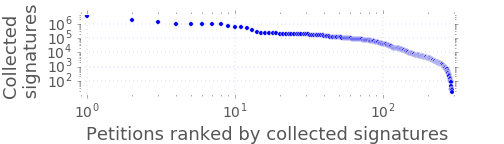
\includegraphics[scale=0.36]{figures/petitionsVSrank.png}
\label{fig:signatures_vs_rank}
\end{SCfigure}


% * Limitation for further exploration                      
\textbf{Tweets with petition:}
To reflect on the second research question we pose in the introduction, it should be noted that petition tweet collection from the campaigns does not account for the overall petition tweet distribution across the whole Twitter. Therefore, we have performed additional collection described below.

To eliminate the bias in a collection of petition tweets, mentioned in the end of the previous paragraph, we have performed an additional request to collect all occurrences of the petition URLs and their redirects. To accomplish this task, we hace preformed extraction similar to the \url{backtweet.com}, which by a given URL returns all occurrences of archived tweets that mention given URL.
Clearly, this still results in only a subset of all possible petition tweets since it does not account for the URL redirects and shortening. However, we aim for a best effort colection which gives us a clearer picture on the distribution of the petitions' distribution on Twitter.
As a result, we have enriched the tweet collection with over 1500 tweets.

\begin{table}[hbt!]
\centering
\begin{tabular}{lcccc}
			& \textit{Successful} & \textit{Failed} &  \textit{Total}	\\ \midrule
Petitions			& 61		& 179		& 240		\\
Proportion			& 26\%		& 74\%		& 100\%		\\
Users 				& 245		& 313		& 558		\\
Tweets				& 601		& 716		& 1317		\\
Goal				& 153093	& 79597		& 116345	\\
Signers				& 170351	& 43739		& 107045	\\ \midrule
\multicolumn{4}{c}{\textit{Petition tweets without campaign hashtags}}	\\ \midrule
Tweets				& 1054		& 707		& 1761		\\
Users 				& 626		& 472		& 1098		\\
\end{tabular}
\caption{\textbf{Global statistics of the petition dataset of environmental campaigns. We show the data for the successful and failed petitions separately, as well as total values and broken links. Users are unique people who tweeted the petition URLs at least once. Additionally, we show average number of tweets collected outside of the campaign hashtag, goal of signatures and number of people who signed for successful and failed petitions. Additionally, we show statistics of the petition tweets that does not had a campaign hashtag.}
\label{tab:petition_tweets}}
\end{table}

\textbf{Dataset preprocessing}
To be able to compare petitions with each other, we use both campaign and non-campaign tweets.
% TODO: Next sentence might be redundant...
For each petition we divide number of obtained signatures by the goal amount and collect various features as described below.
Thus a petition $p$ is characterized by its signatures goal $S(p)$, collected signatures $C(p)$, and set of Twitter related features $T_i(p)$, e.g., (1) Number of unique users posted the petition url, (2) Number of tweets with url, (3) Number of followers of the users posting petition tweets, (4) Number of tweets with campaign hashtags vs without.